Il seguente codice MatLab, riguarda la funzione $\theta_{h}(x) = \frac{f(x+h)-f(x-h)}{2h}$, indicando con $h=10^-j$, $j=1,...,10$, $f(x)=x^4$ e $x=1$ :\\
	\lstinputlisting[language=Matlab]{Cap_1/Es_3/Es_3.m}
restituisce i seguenti valori:\\
\begin{center}
	\begin{tabular}{|c|c|}
		\hline
			$h$ & $\theta_{h}(1)$  \\
		\hline
    		\(10^{-1}\) & $4.040000000000002e+00$\\
    		\(10^{-2}\) & $4.000400000000004e+00$\\
    		\(10^{-3}\) & $4.000003999999723e+00$\\
    		\(10^{-4}\) & $4.000000039999230e+00$\\
    		\(10^{-5}\) & $4.000000000403681e+00$\\
    		\(10^{-6}\) & $3.999999999948489e+00$\\
    		\(10^{-7}\) & $4.000000000115023e+00$\\
    		\(10^{-8}\) & $4.000000003445692e+00$\\
    		\(10^{-9}\) & $4.000000108916879e+00$\\
    		\(10^{-10}\) & $4.000000330961484e+00$\\
		\hline
	\end{tabular}
\end{center} 
Si vede che i valori di $\theta_{h}(1)$ diminuiscono fino ad $h = 10^{-6}$, in cui si ha il minimo valore di $\theta_{h}(1)$, dopodichè inizia a crescere. Mostriamo l'andamento relativo nel seguente plot:
\begin{figure}[H]
	\label{Cap_1_Es_3}
	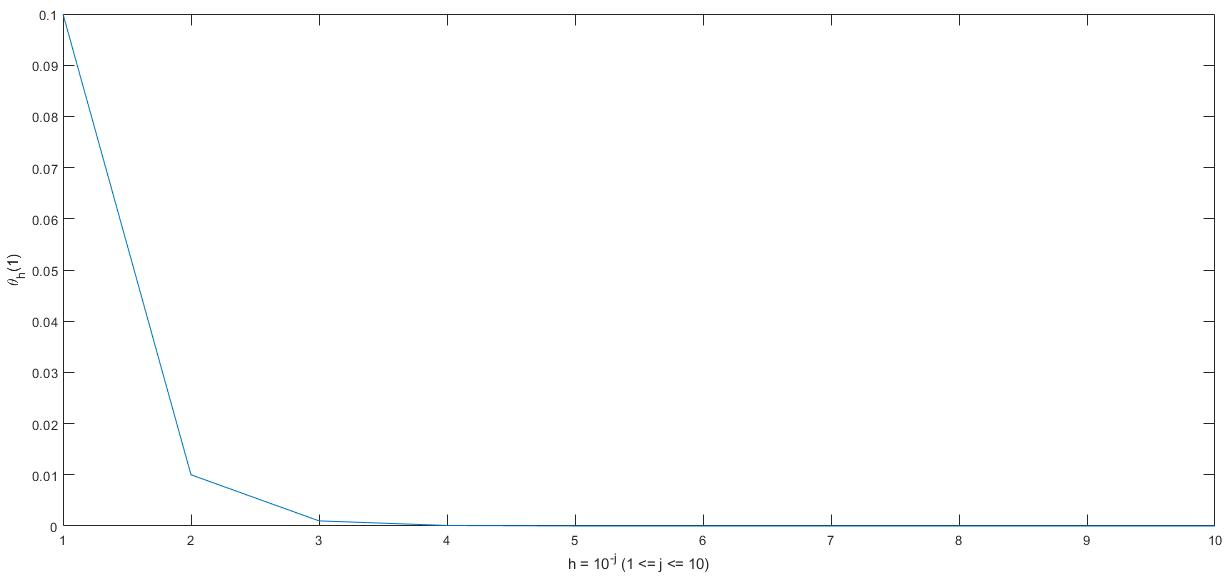
\includegraphics[width=\textwidth]{Plot/Cap_1_Es_3}
		\caption{Andamento della funzione $\theta_{h}(1)$}
\end{figure}